\section{Background}

\begin{frame}{Literature and Context}
  \begin{itemize}
    \item Stream 1: summarize the benchmark literature, for example \textcite{blanchard2017macroeconomics}.
    \item Stream 2: explain the unresolved gap.
    \item Stream 3: position your approach or data relative to \textcite{akerlof2000near}.
  \end{itemize}
\end{frame}

\begin{frame}{Stylized Facts}
  \begin{figure}
    \centering
    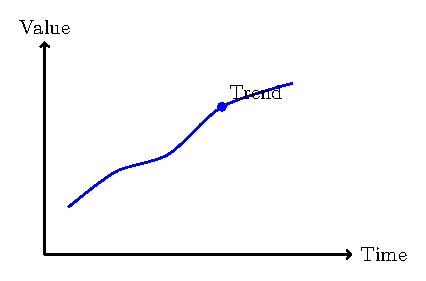
\includegraphics[width=0.74\linewidth,height=0.56\textheight,keepaspectratio]{figures/example-chart.pdf}
    \caption{Replace with your core descriptive figure.}
  \end{figure}
\end{frame}
